%%%%%%%%%%%%%%%%%%%%%%%%%%%%%%%%%%%%%%%%%%%%%%%%

\documentclass[12pt, a4paper]{report}
\usepackage[latin1]{inputenc}
\usepackage{amsmath}
\usepackage{amsfonts}
\usepackage{amssymb}
\usepackage{graphicx}
\usepackage{booktabs}
\usepackage[export]{adjustbox}
\usepackage[style=apa, backend=biber]{biblatex}

%%%%%%%%%%%%%%%%%%%%%%%%% ADD ANY ADDITIONAL PACKAGES BELOW
% Uncomment for blank lines between paragraphs rather than
% indents
\usepackage[parfill]{parskip}

%%%%%%%%%%%%%%%%%%%%%%%%%%%%%%%%%%%%%%%%%%%%%%%%%%%%%%%%%%%%


%%%%%%%%%%%%

\addbibresource{refs.bib}

\usepackage[linktocpage=true]{hyperref}	% This creates hyperlinks and moves the contents links to the page number for clarity
% There are lots of options you can alter to what you want, see http://www.tug.org/applications/hyperref/manual.html
\usepackage[font=small,labelfont=bf]{caption}	% This ensures hyperlinks to figures link to the top of the figure not the caption. This line must come after the previous one (hyperref package).
\linespread{1.3}


\begin{document}
\pagenumbering{alph}	% This stops the title page being counted in the page numbering
\thispagestyle{empty}	% This stops a number being put at the bottom
\vspace*{1mm}	% The asterisk is needed because it's at the top of a page

\includegraphics[width=0.7\textwidth, right]{figures/UoP_Primary_Logo_Stacked_pms.eps}
\vspace{10mm}

\begin{center}
% Put the full title  on the front page
\huge\textbf{\textsf{Insert Dissertation\\Title Here}}\\
\vspace{15mm}
% The student handbook states you need your full name on the front page
\large \textbf{Insert Author Here}\\


\vspace{10mm}
\normalsize School of Computing \\ Final Year Project PJE / PJS 40

\vspace{20mm}
%
\today	% This prints todays date, eg. ``January 1, 2012``.
% Make sure all of the above fits on the front page, otherwise you will have to change the spacings, eg. to accomodate a long title
\end{center}
\newpage
\pagenumbering{roman}	% This sets page numbers to be Roman numerals for the preliminaries
\phantomsection	% This makes the abstract's bookmark link to the top of the page instead of the title line.
\addcontentsline{toc}{chapter}{Abstract}	% Gives the Abstract a contents entry
\chapter*{Abstract}	% The asterisk stops a chapter number being assigned

No more than 300 words summarizing this dissertation.

\newpage
\renewcommand{\contentsname}{Table of Contents}	% Changes the contents title from 'Contents' to 'Table of Contents' just because it looks better.
\pdfbookmark{Table of Contents}{contents}	% Adds a bookmark 'Table of Contents' in the PDF and labelled 'contents' for the hyperref package.
\tableofcontents

\newpage
\pdfbookmark{List of Tables}{tables}	% Adds a bookmark 'List of Tables' in the PDF and labelled 'tables' for the hyperref package.
\listoftables

\newpage
\pdfbookmark{List of Figures}{figures}	% Adds a bookmark 'List of Figures' in the PDF and labelled 'figures' for the hyperref package.
\listoffigures

% The commands for the preliminary sections below serve the same purposes as for the abstract section above, You can add or remove sections as you see fit.
% Here might also be a good place to put a dedication if you want.
%\newpage
%To...

\newpage

\phantomsection
\addcontentsline{toc}{chapter}{Acknowledgements}
\chapter*{Acknowledgements}
Thanks.
\newpage


\pagenumbering{arabic}	% Begins normal page numbering for the body of the report.


%%%%%%%%%%%%%%%%% INCLUDE YOUR CHAPTERS BELOW
% If you move the order around, all the cross references remain, sensibly renumbered.
% yay!
\chapter{Introduction} \label{chap:intro}
A gentle reminder not to get this chapter perfect until the dissertation is nearing its completion\ldots

\section{A section}

\subsection{A sub-section}

\subsubsection{A sub-sub-section}



\section{Citations}

When it comes to referencing, if we want to assert a fact and then provide its reference use \verb!\parencite!. For example -- one should adapt feedback to learner personality \parencite{dennis2016adapting}.

Or if you want to talk about the research directly, use \verb!\textcite!: \textcite{dennis2016adapting} did a PhD in adapting feedback to learner personality. 

If you want to cite two sources at the same time, you can separate the keys with commas \parencite{dennis2016adapting,cle12}.

\section{Figures}

\begin{figure}
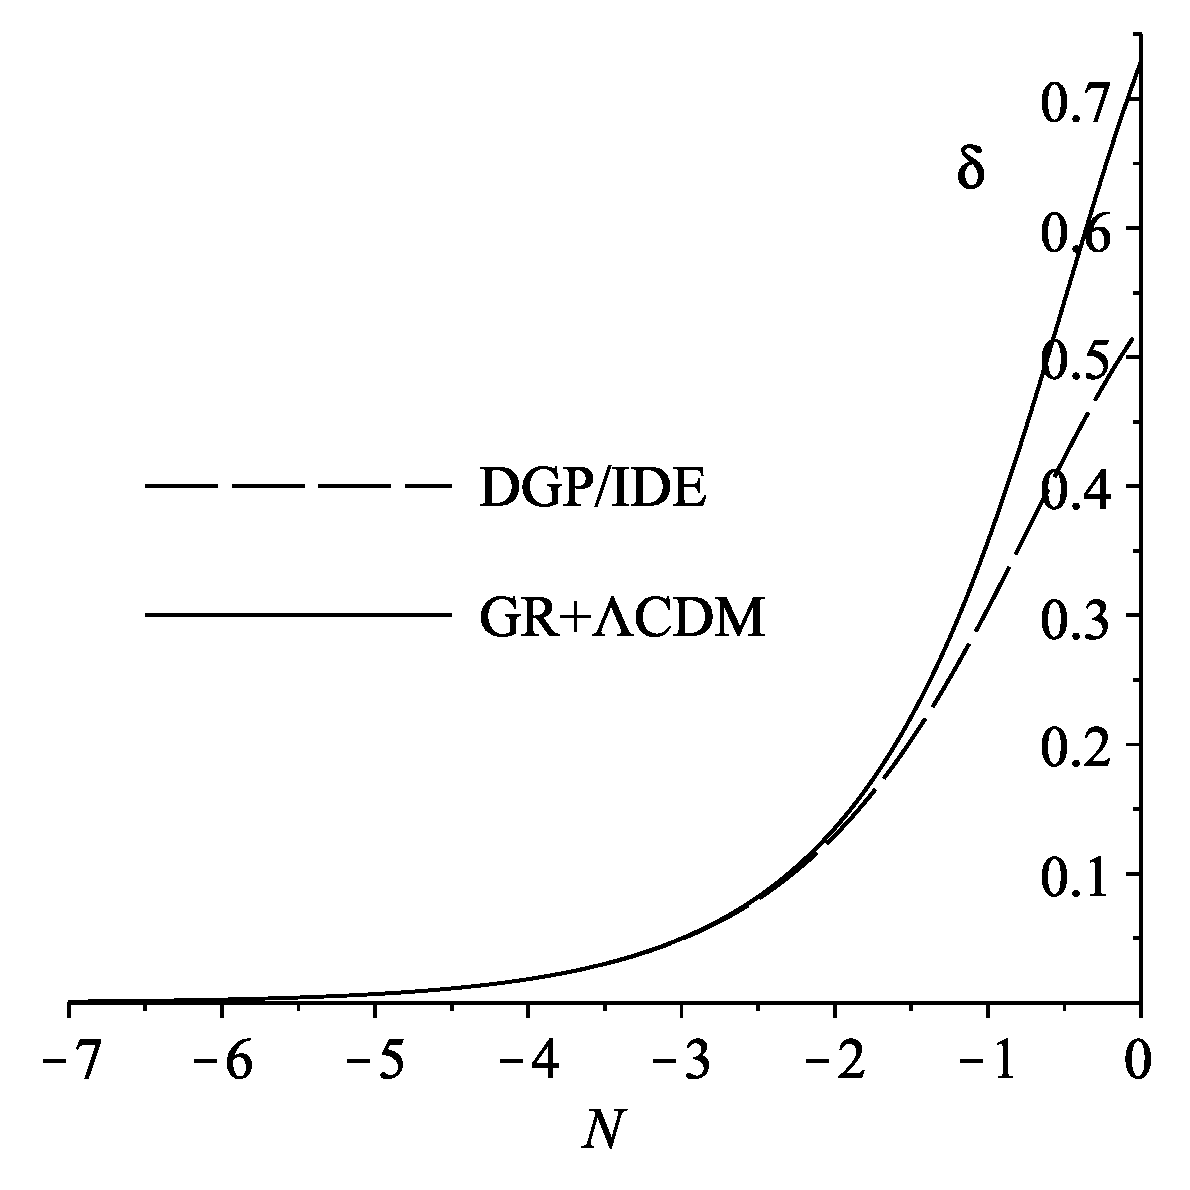
\includegraphics[width=0.49\columnwidth]{figures/dgpdeltas.eps}
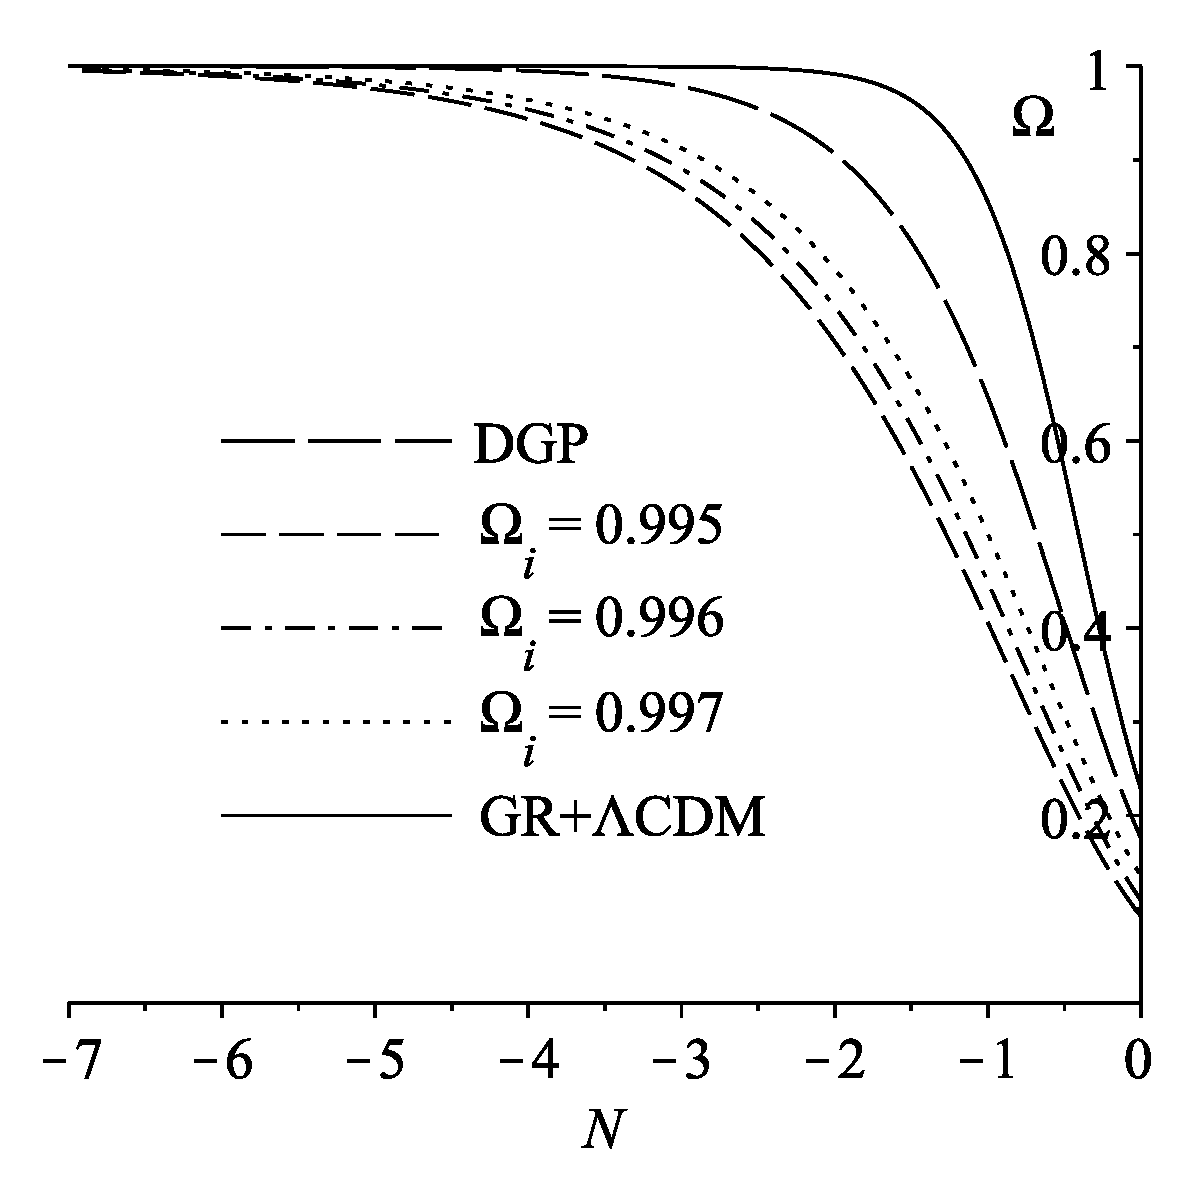
\includegraphics[width=0.49\columnwidth]{figures/dgpomegas.eps}
% For long captions include a short version for the List of Figures/Tables sections in square brackets as below.
\caption[Evolutions of $\delta$ and $\Omega$ for DGP]{Evolution of the density perturbation (left) and the density parameters (right) for the matched DGP/IDE models, each with a different $\Omega_i$,
and a GR+$\Lambda$CDM model.
\label{fig:matched}}
\end{figure}

Don't the graphs in \autoref{fig:matched} look scary? Don't worry, this is because I adapted this template from ICJS. Remember - if you are including screenshots or other raster graphics (i.e. PNG, JPEG) you should ensure that they are at least 300dpi. This will take effort on your part - most people's screens are at 72dpi.   

Vector is better (EPS or PDF) if you can manage it. If you are exporting graphs from Microsoft Excel for example, place the chart in its own sheet and print it to PDF. Then, using Acrobat or similar, crop the whitespace off the PDF. This is the most reliable way I have found to include vector graphics from Microsoft Office.







% To include math symbols in things with hyperlinks you need to specify an alternative plain text version for the bookmark using \texorpdfstring as below:
\section{A section with math symbols, eg. \texorpdfstring{$\Lambda$}{Lambda}CDM}
test test test test test test test test test test test test test test test test test test test test test test test test test test test test test test test test test test test test test test test test
test test test test test test test test test test test test test test test test test test test test test test test test test test test test test test test test test test test test test test test test
test test test test test test test test test test test test test test test test test test test test test test test test test test test test test test test test test test test test test test test test
test test test test test test test test test test test test test test test test test test test test test test test test test test test test test test test test test test test test test test test test



\chapter{More examples}

\section{Equations}

Here's an equation,
\begin{equation}
E=mc^2.\label{eq:einstein}
\end{equation}

\noindent I can reference that easily in the text: \autoref{eq:einstein}. It's even a hyperlink. How nice. 

\section{Opening and closing quotes}

Unlike modern word processors, you need to specify in \LaTeX{} which quote mark to print. To get an opening quote you use a backtick and the regular apostrophe for a closing quote. Double them up for speech. ``This isn't so hard after all''. One just needs to `get used' to it. 

One should never use an apostrophe for plurals. Nope, not even for abbreviations, e.g. in the 1990s, people bought CDs from Virgin Megastores. 

In the \textbf{extremely} rare cases where it's unclear, match it with an opening quote if you must. I got three `A's for my AS Levels. 

\section{Tables}

Tables are joyous fun. The \verb+tabular+ environment is the most common, although it's rather old fashioned and wrangling it into doing what you want can be arcane. Happily, tablesgenerator.com can produce tables from a visual editor or paste from word.

A few things to help you unlearn bad table habits:

\begin{itemize}
    \item You should not use vertical lines in tables. Seriously -- this is an awful 1990s era default from Microsoft Word which has hung around and never gone away. 
    \item the booktabs package can make prettier tables (vertical lines are intentionally banned) - select this option in tablesgenerator. I have included the package for you
    \item You should use tables for comparing numerical data and not as a way of laying out content or paragraph text
\end{itemize}

\begin{table}
    \centering
    \begin{tabular}{lccc}
        \toprule
        \textbf{Feature} & \textbf{Liked (\%)} & \textbf{Disliked (\%)} & \textbf{Didn't know (\%)}  \\ \midrule
        Vertical lines & 0 & 90 & 10 \\
        Using Word & 40 & 40 & 20 \\
        \bottomrule
    \end{tabular}
    \caption{Made up percentages of participants that liked random features}
    \label{tab:sample}
\end{table}

\noindent \autoref{tab:sample} shows a simple table made by hand by yours truly. Note that the column separator is \& which means you must always escape that character if you want to use it in text.





%%%%%%%%%%%%%%% APPENDICES
\appendix
\chapter{First Appendix}


%%%%%%%%%%%%%% REFERENCES SECTION
\newpage
\phantomsection
\addcontentsline{toc}{chapter}{Bibliography}
% In order to try and get a consistent format I copy and paste the INSPIRE bibtex code into my bibtex file.
\printbibliography



\end{document}
